
\setcounter{chapter}{3}
\chapter{Sprint 2: User and App Managment}
\minitoc %insert la minitoc
\graphicspath{{Chapter4/figures/}}

%\DoPToC
%==============================================================================
\pagestyle{fancy}
\fancyhf{}
\fancyhead[R]{\bfseries\rightmark}
\fancyfoot[R]{\thepage}
\renewcommand{\headrulewidth}{0.5pt}
\renewcommand{\footrulewidth}{0pt}
\renewcommand{\chaptermark}[1]{\markboth{\MakeUppercase{\chaptername~\thechapter. #1 }}{}}
\renewcommand{\sectionmark}[1]{\markright{\thechapter.\thesection~ #1}}

\begin{spacing}{1.2}

%==============================================================================
\section*{Introduction}
In order to integrate Flouci as a web payment method, we opted for an app model. This model consists of creating an app for each integration the developer wants to have, the app contains basic information about the e-commerce website and it's also linked to a Flouci account to accept payment directly.
\newline
In this chapter, we will start our project development. We will focus on implementing two linked parts of our application which are the user and app. 

\section{Database}
Our database modal can be divided into three big sections of the projects. We have tables managing the user data, Tables managing the app data and others independent tables handling auditing events. Also, we made the modal in a way that the user can have from 0 to N apps and an app can only be linked to one user.
The database schema is presented in the figure \ref{fig:database}
\begin{figure}[H]\centering
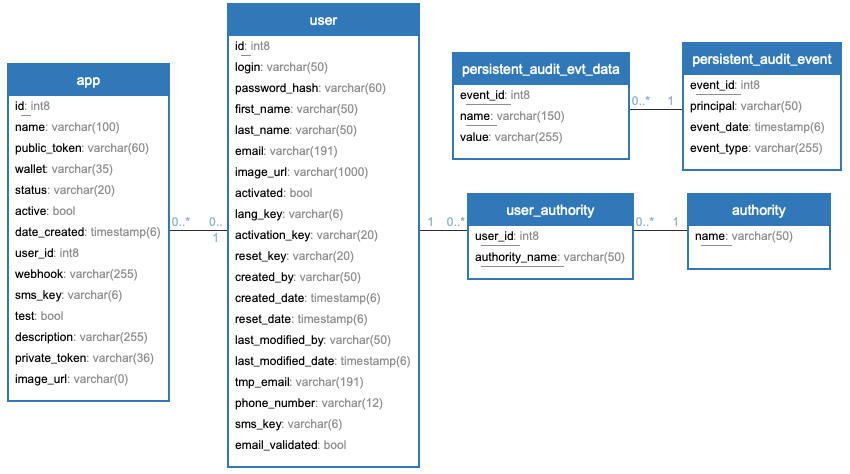
\includegraphics[scale=0.6]{db.png}
\caption{Database modal}
\label{fig:database}
\end{figure}


\section{User Management}
In this section we will explain our user management strategy, the mechanism of creating the account and the different authorities used. we also present how to recover a lost account.
\subsection{Authorities}
In our project we used four different authorities to manage access to different parts of the app:
\begin{itemize}
	\item \textbf{System}: who is mainly used by our audit logs, when something is done automatically
	\item \textbf{AnonymousUser:} who is given to anonymous users when they do an action
	\item \textbf{Developer}: who is a normal user with 'ROLE\_DEVELOPER' authorization it gives access to managing apps.
	\item  \textbf{Admin}: who is an admin user with 'ROLE\_DEVELOPER' and 'ROLE\_ADMIN' authorizations, he can manage users.
\end{itemize}

\subsection{Registration}
The registration process is very simple. we only require basic info and a valid email address to open an account. All created accounts have a "DEVELOPER" authorities which basically give them access to restricted functionalities. 

We only activate the user account after the email confirmation. The activation email contains a link with a key saved in the database. Accessing the link will activate the account.

The figure \ref{fig:register} is a sequence diagram that presents all the step needs to create a new account.

\begin{figure}[H]\centering
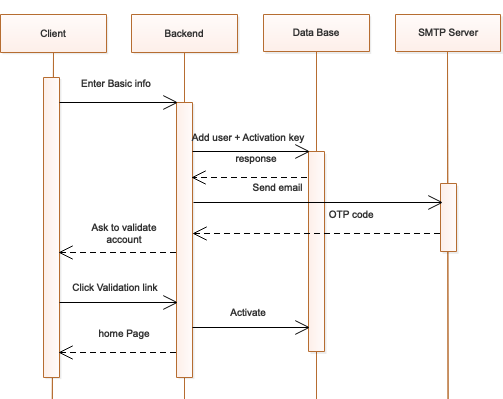
\includegraphics[scale=0.8]{Register_user_sequence_diagram.png}
\caption{User Registration Sequence diagram}
\label{fig:register}
\end{figure}



\subsection{Recover Account}
In case the user forgets his password, he can simply reset it by email. we attach a key to the request and we send the URL with the key to the email. The link with the key takes the user to a page where he can put a new password. After that our backend check the reset key and apply the changes.

\section{App Management}
In our project each e-commerce website is linked to an app to be able to accept Flouci as a payment method.
In this section we will explain key functionalities of the app.
\subsection{App Creation}
Every app is linked to a Flouci Merchant account. Besides the basic information, the developer should enter a phone number to identify the Flouci account then confirm it with the OTP key he gets by SMS.

After finishing creating the app, the developer will obtain two tokens.

The figure \ref{fig:appcreate} shows the whole process in details.
\begin{figure}[H]\centering
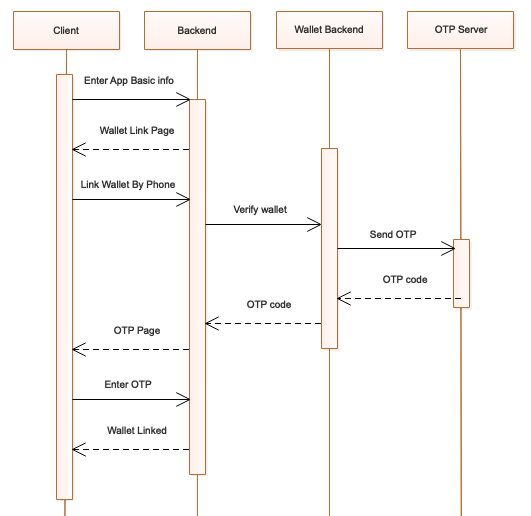
\includegraphics[scale=0.7]{Create_App_Sequence_Diagram.png}
\caption{App creation Sequence diagram}
\label{fig:appcreate}
\end{figure}
\subsection{App Revoke}
Since the app have two main tokens (public and private), we offer the possibility to revoke an app simply by changing its public token. Changing the token will result in obsoleting all current integration of the app since they all will be using a public token that doesn't resolve our app.

\subsection{App Metrics}
After the integration, there is a huge  risk of the developer shifting a way of the platform. We decided to gather metrics for the user to be able to bring him back to the platform.
Each app have two main metrics.
\begin{itemize}
	\item \textbf{Transactions:} the number of orders made.
	\item \textbf{Gross sales:} the total amount of all orders.
\end{itemize}
We also save the metrics per day with a cron job, so we can easily create charts to monitor sales.

\subsection{Orders}
With every online payment, we attach the app id to the payment payload. This information will help us get the list of orders for each app.
We can then display all orders made, add filtering and even add a button to reimburse orders.

\section*{Conclusion}
In this section, we implemented the first steps the user should do in order to integrate Flouci. After creating an account and an app, The two tokens provided will be the only missing piece to integrate Flouci payment method.

In the next section, we will implement the checkout API which can be integrated into any e-commerce website.
%==============================================================================
\end{spacing}
